\item \points{40} {\bf Linear Classifiers (logistic regression and GDA)}

In this problem, we cover two probabilistic linear classifiers we have
covered in class so far. First, a discriminative linear classifier: logistic
regression. Second, a generative linear classifier: Gaussian discriminant
analysis (GDA). Both the algorithms find a linear decision boundary that
separates the data into two classes, but make different assumptions. Our goal
in this problem is to get a deeper understanding of the similarities and
differences (and, strengths and weaknesses) of these two algorithms.

For this problem, we will consider two datasets, along with starter codes provided in the following
files:
\begin{center}
\begin{itemize} %[label=\roman*.]
	\item \url{src/linearclass/ds1_{train,valid}.csv}
	\item \url{src/linearclass/ds2_{train,valid}.csv}
        \item \url{src/linearclass/logreg.py}
        \item \url{src/linearclass/gda.py}
\end{itemize}
\end{center}
Each file contains $\nexp$ examples, one example $(x^{(i)}, y^{(i)})$ per row.
In particular, the $i$-th row contains columns $x^{(i)}_0\in\Re$,
$x^{(i)}_1\in\Re$, and $y^{(i)}\in\{0, 1\}$. In the subproblems that follow, we
will investigate using logistic regression and Gaussian discriminant analysis
(GDA) to perform binary classification on these two datasets.

\begin{enumerate}
	\item \subquestionpoints{10}

%\textbf{TBD RETIRE THIS QUESTION? Q4c is a more generic version of this}

In lecture we saw the average empirical loss for logistic regression:
\begin{equation*}
	J(\theta)
	= -\frac{1}{\nexp} \sum_{i=1}^\nexp \left(y^{(i)}\log(h_{\theta}(x^{(i)}))
		+  (1 - y^{(i)})\log(1 - h_{\theta}(x^{(i)}))\right),
\end{equation*}
where $y^{(i)} \in \{0, 1\}$, $h_\theta(x) = g(\theta^T x)$ and
$g(z) = 1 / (1 + e^{-z})$.

Find the Hessian $H$ of this function, and show that for any vector $z$, it
holds true that
%
\begin{equation*}
    z^T H z \ge 0.
\end{equation*}
%
{\bf Hint:} You may want to start by showing that
$\sum_i\sum_j z_i x_i x_j z_j = (x^Tz)^2 \geq 0$. Recall also that
$g'(z) = g(z)(1-g(z))$.

{\bf Remark:} This is one of the standard ways of showing that the matrix $H$
is positive semi-definite, written ``$H \succeq 0$.''  This implies that $J$ is
convex, and has no local minima other than the global one. If you have some
other way of showing $H \succeq 0$, you're also welcome to use your method
instead of the one above.


        \ifnum\solutions=1 {
            \begin{answer}

\[J(\theta) = -\frac{1}{\nexp} \sum_{i=1}^\nexp \left(y^{(i)}\log(h_{\theta}(x^{(i)})) +  (1 - y^{(i)})\log(1 - h_{\theta}(x^{(i)}))\right)\]
\[\frac{\partial J(\theta)}{\partial x_i} = \Sigma-(y - h(x)x_i\]
\[H_i_j =  \frac{\partial^2 J(\theta)}{\partial x^2}\] 
\[=\Sigma(\frac{\partial h(x)}{\partial \theta_j)}x_i  \]
\[=\Sigma (h(x)(1 - h(x)) x_jx_i \]
		Assume
\[x_ix_j = X_i_j \]  
\[=\Sigma (h(x)(1 - h(x)) xx^T\]

\[z^THz \geq 0\]
		is always positive-semidefinite when H \geq 0
		
\[z^THz =  z^T(\Sigma (h(x)(1 - h(x)) xx^T)z\]
\[=\Sigma (h(x)(1 - h(x)) (z^Txx^Tz)\]
\[=\Sigma (h(x)(1 - h(x)) (x^Tz)^2\]

\[(x^Tz)^2\]  
 		is positive, and \[h(x)(1 - h(x)\] 
 		is a bernoulli probability 
 where:
\[0 \leq h(x) \leq 1\] 
 Therefore, the value of that replaces the hessian determines whether $z^THz$  is positive semidefinite, or negative semidefinite. In this case the Hessian is positive semidefinite.
So, 
\[z^THz \geq 0\]

\end{answer}


        } \fi

	\item \subquestionpoints{5} \textbf{Coding problem.}
Follow the instructions in \texttt{src/linreg/logreg.py} to train a
logistic regression classifier using Newton's Method.
Starting with $\theta = \vec{0}$, run Newton's Method until the updates to
$\theta$ are small: Specifically,  train until the first iteration $k$ such
that $\|\theta_{k} - \theta_{k-1}\|_1 < \epsilon$, where
$\epsilon = 1\times 10^{-5}$. Make sure to write your model's predicted probabilities on
the validation set to the file specified in the code.

Include a plot of the \textbf{validation data} with $x_1$ on the horizontal axis and $x_2$ on the vertical axis.
To visualize the two classes, use a different symbol for examples $x^{(i)}$
with $y^{(i)} = 0$ than for those with $y^{(i)} = 1$. On the same figure, plot the decision boundary
found by logistic regression (i.e, line corresponding to $p(y|x) = 0.5$).


        \ifnum\solutions=1 {
            \begin{answer}

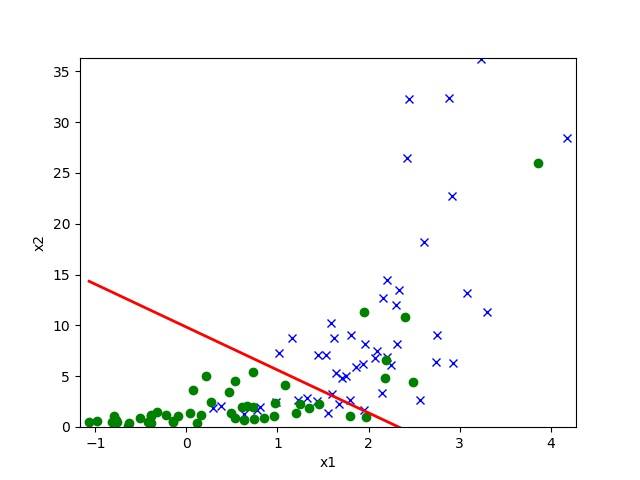
\includegraphics{logreg_pred_1.hpg}

\end{answer}

        } \fi


	\item \subquestionpoints{5}
Recall that in GDA we model the joint distribution of $(x, y)$ by the following
equations:
%
\begin{eqnarray*}
	p(y) &=& \begin{cases}
	\phi & \mbox{if~} y = 1 \\
	1 - \phi & \mbox{if~} y = 0 \end{cases} \\
	p(x | y=0) &=& \frac{1}{(2\pi)^{\di/2} |\Sigma|^{1/2}}
		\exp\left(-\frac{1}{2}(x-\mu_{0})^T \Sigma^{-1} (x-\mu_{0})\right) \\
	p(x | y=1) &=& \frac{1}{(2\pi)^{\di/2} |\Sigma|^{1/2}}
		\exp\left(-\frac{1}{2}(x-\mu_1)^T \Sigma^{-1} (x-\mu_1) \right),
\end{eqnarray*}
%
where $\phi$, $\mu_0$, $\mu_1$, and $\Sigma$ are the parameters of our model.

Suppose we have already fit $\phi$, $\mu_0$, $\mu_1$, and $\Sigma$, and now
want to predict $y$ given a new point $x$. To show that GDA results in a
classifier that has a linear decision boundary, show the posterior distribution
can be written as
%
\begin{equation*}
	p(y = 1\mid x; \phi, \mu_0, \mu_1, \Sigma)
	= \frac{1}{1 + \exp(-(\theta^T x + \theta_0))},
\end{equation*}
%
where $\theta\in\Re^\di$ and $\theta_{0}\in\Re$ are appropriate functions of
$\phi$, $\Sigma$, $\mu_0$, and $\mu_1$.


        \ifnum\solutions=1 {
            \begin{answer}


Given that:
\[p(y\vert x) = \frac{p(x\vert y) p(y)}{p(x)}\]
\[p(y = 1\vert x; \phi, \mu_0, \mu_1, \Sigma)
\[=\frac{p(x\vert y=1; \phi, \mu_0, \mu_1, \Sigma)p(y=1; \phi, \mu_0, \mu_1, \Sigma)}{p(x;\phi,\mu_0,\mu_1,\Sigma)}\]
\[=\frac{p(x\vert y=1)p(y=1)}{p(x)}\]
\[= \frac{p(x\vert y=1)p(y=1)}{p(x\vert y= 0)p(y=0)+p(x\vert y=1)p(y=1)}\]
\[=\frac{exp(\frac{-1}{2}(x-\mu_1)^T\Sigma^-1(x-\mu_1))(\phi)}{exp(\frac{-1}{2}(x-\mu_0)^T \Sigma^-1 (x-\mu_0))(1-\phi) + exp(\frac{-1}{2}(x-\mu_1)^T \Sigma^-1 (x-\mu_1))(\phi)}\]
\[= \frac{1}{1+\frac{1-\phi}{\phi}exp(\frac{-1}{2}(x-\mu_0)^T \Sigma^-1 (x-\mu_0) + \frac{1}{2}(x-\mu_1)^T \Sigma^-1 (x-\mu_1)}\]
\[=\frac{1}{1 + exp(\frac{-1}{2}((x-\mu_0)^T \Sigma^-1\mu_0 -\mu_1)^T \Sigma^-1 \mu_1) + log(\frac{1-\phi}{\phi}))}\]

rearranging terms
\[ (x - \mu_0)^T \Sigma^-1(x-\mu_0) - (x-\mu_1)^T \Sigma^-1(x-\mu_1) \]
\[= x^T\Sigma^-1 x - \mu_0^T \Sigma^-1 x - x^T \Sigma^-1 \mu_0 + \mu_0^T \Sigma^-1 \mu_0 - x^T \Sigma^-1 x + \mu_1^T \Sigma^-1 x + x^T \Sigma^-1 \mu_1 - \mu_1^T \Sigma^-1 \mu_1 \]
\[= -2 \mu_0^T \Sigma^-1 x + \mu_0^T \Sigma^-1 \mu_0 + 2 \mu_1^T \Sigma^-1 c - \mu_1^T \Sigma^-1 \mu_1 \]
\[= 2(\mu_1 - \mu_0)^T \Sigma^-1 x + \mu_0^T \Sigma^-1 \mu_0 - \mu_1^T \Sigma^-1 \mu_1 \]
Therefore: 
\[p(y = 1\vert x; \phi, \mu_0, \mu_1, \Sigma) = \[=\frac{1}{1 + exp(log \frac{1-\phi}{phi} + \frac{1}{2} \mu_1^T \Sigma^-1 \mu_1 - \frac{1}{2} \mu_0^T \Sigma^-1 \mu_0 + (\mu_0 - \mu_1)^T \Sigma^-1 x}\]
The term inside the exp can be expressed as a linear function
\[ \theta = \Sigma^-1 (\mu_1 - \mu_0) \]
\[ \theta_0 = \frac{1}{2}(\mu_0^T \Sigma^-1 \mu_0 - \mu_1 ^T \Sigma^-1 \mu_1) - log \frac{1-\phi}{\phi}
\end{answer}

        }\fi

	\item \subquestionpoints{7} Given the dataset, we claim that the maximum
  likelihood estimates of the parameters are given by
  \begin{eqnarray*}
    \phi &=& \frac{1}{\nexp} \sum_{i=1}^\nexp 1\{y^{(i)} = 1\} \\
\mu_{0} &=& \frac{\sum_{i=1}^\nexp 1\{y^{(i)} = {0}\} x^{(i)}}{\sum_{i=1}^\nexp
1\{y^{(i)} = {0}\}} \\
\mu_1 &=& \frac{\sum_{i=1}^\nexp 1\{y^{(i)} = 1\} x^{(i)}}{\sum_{i=1}^\nexp 1\{y^{(i)}
= 1\}} \\
\Sigma &=& \frac{1}{\nexp} \sum_{i=1}^\nexp (x^{(i)} - \mu_{y^{(i)}}) (x^{(i)} -
\mu_{y^{(i)}})^T
  \end{eqnarray*}
  The log-likelihood of the data is
  \begin{eqnarray*}
\ell(\phi, \mu_{0}, \mu_1, \Sigma) &=& \log \prod_{i=1}^\nexp p(x^{(i)} , y^{(i)};
\phi, \mu_{0}, \mu_1, \Sigma) \\
&=& \log \prod_{i=1}^\nexp p(x^{(i)} | y^{(i)}; \mu_{0}, \mu_1, \Sigma) p(y^{(i)};
\phi).
  \end{eqnarray*}
By maximizing $\ell$ with respect to the four parameters,
prove that the maximum likelihood estimates of $\phi$, $\mu_{0}, \mu_1$, and
$\Sigma$ are indeed as given in the formulas above.  (You may assume that there
is at least one positive and one negative example, so that the denominators in
the definitions of $\mu_{0}$ and $\mu_1$ above are non-zero.)


        \ifnum\solutions=1 {
            \begin{answer}


Introducing formulas 
\[\sum \log p(x^i \mid y^i ; \mu_0, \mu_1, \Sigma) + \Sigma \log p(y^i; \phi) \]
\[ \Sigma [ \frac{1}{2}\log\frac{1}{\Sigma} -\frac{1}{2}(x^i - \mu_y)^T \Sigma^-1 (x^i - \mu_y ) + y^i\log(\phi) + (1-y^i) * \log(1-\phi)]

wrt phi
\begin{eqnarray*}
\[ \frac{\partial\ell}{\partial\phi} &=& \Sigma (\frac{y^i}{\phi} - \frac{1-y^i}{1-\phi}) \] \\
\[  \frac{\Sigma  1* [y^1 = 1]} {\phi} - \frac{n- \Sigma 1* [y^1 = 1]}{1-\phi} \\ \]
\[ \phi &=& \frac{1}{n} \Sigma{1* [y^i = 1]} \]
\end{eqnarray*}
wrt mu0 and mu1

\begin{eqnarray*}
\frac{\partial\ell}{\partial\mu_0} &=& -\frac{1}{2} \Sigma \frac{\partial}{\partial\mu_0} (x^i - \mu_0)^T \Sigma^-1 (x^i - \mu_0) \\
&=& -\frac{1}{2} \Sigma \frac{\partial}{\partial\mu_0} [\mu_0^T\Sigma^-1\mu_0 - x^i\Sigma^-1\mu_0 - \mu_0^T\Sigma^-1 x^i] \\
&=& -\frac{1}{2} \Sigma \frac{\partial}{\partial\mu_0} tr[\mu_0^T\Sigma^-1\mu_0 - x^i\Sigma^-1\mu_0 - \mu_0^T\Sigma^-1 x^i] \\
&=& -\frac{1}{2} \Sigma [2\Sigma^-1 \mu_0 - 2\Sigma^-1 x^i]
\end{eqnarray*}

For Sigma
\begin{eqnarray*}
\[\frac{\partial\ell}{\partial\Sigma} &=& \Sigma \frac{\partial}{\partial\Sigma}[ \frac{1}{2}\log\frac{1}{\Sigma} - \frac{1}{2}(x^i - \mu_y)^T 	\frac{1}{\Sigma}(x^i - \mu_y)] \\ &=&  \Sigma \frac{1}{2}\Sigma {\partial}{\partial\Sigma}\frac{1}{\Sigma} - \frac{1}{2} \frac{\partial}{\partial\Sigma} (x^i - \mu_y)^T 	\frac{1}{\Sigma}(x^i - \mu_y)] \\
	&=& \Sigma \frac{1}{2} {\partial}{\partial\Sigma}\frac{1}{\Sigma}\Sigma^T - \frac{1}{2} \frac{\partial}{\partial\Sigma} (x^i - \mu_y)^T(x^i - \mu_y)] \\
	&=& \Sigma[\frac{1}{2}[\frac{1}{\Sigma}]^-1 - \frac{1}{2}(x^i - \mu_y)*(x^i - \mu_y)^T] \\
	&=& \frac{1}{2}\Sigma[\Sigma - (x^i - \mu_y)*(x^i - \mu_y)^T]
\end{eqnarray*}

\end{answer}

        } \fi

	\item \subquestionpoints{5} \textbf{Coding problem.}
In \texttt{src/linreg/gda.py}, fill in the code to
calculate $\phi$, $\mu_{0}$, $\mu_{1}$, and $\Sigma$, use these parameters
to derive $\theta$, and use the resulting GDA model to make predictions on the
validation set. Make sure to write your model's predictions on
the validation set to the file specified in the code.

Include a plot of the \textbf{validation data} with $x_1$ on the horizontal axis and $x_2$ on the vertical axis.
To visualize the two classes, use a different symbol for examples $x^{(i)}$
with $y^{(i)} = 0$ than for those with $y^{(i)} = 1$. On the same figure, plot the decision boundary
found by GDA (i.e, line corresponding to $p(y|x) = 0.5$).


        \ifnum\solutions=1 {
            \begin{answer}

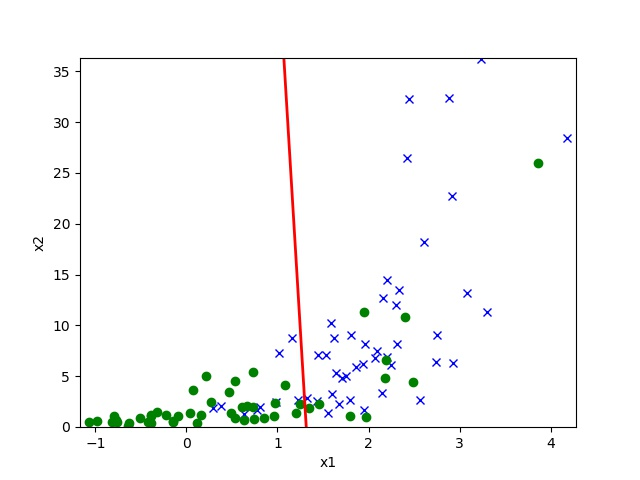
\includegraphics{gda_pred_1.jpg}
 
\end{answer}

        } \fi

	\item \subquestionpoints{2}
For Dataset 1, compare the validation set plots obtained in part (b) and part (e)
from logistic regression and GDA respectively, and briefly comment on your observation
in a couple of lines.


        \ifnum\solutions=1 {
            \begin{answer}

The model with logistic regression shows a closer approximation, and provides a good fit to the validation set.
The GDA model does not fit the data as well as LOG REG.

\end{answer}

        } \fi

	\item \subquestionpoints{5}
Repeat the steps in part (b) and part (e) for Dataset 2. Create similar plots on
the \textbf{validation set} of Dataset 2 and include those plots in your writeup.

On which dataset does GDA seem to
perform worse than logistic regression? Why might this be the case?


        \ifnum\solutions=1{
            \begin{answer}

Both plots look identical, and both models fit the validation set equally well. 
This is the case because the data in the dataset 2 is more separated, so both algorithms produce a good separation.

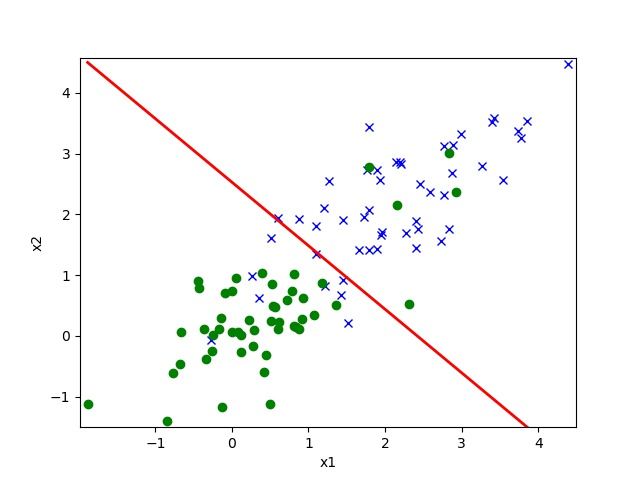
\includegraphics{logreg_pred_2.jpg}

for log reg dataset 2

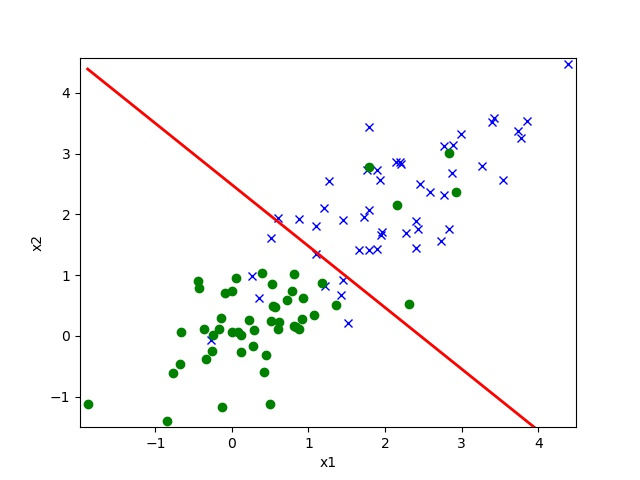
\includegraphics{gda_pred_2.jpg}

for gda dataset 2

\end{answer}
        }\fi

	\item \points{1} For the dataset where GDA performed worse in
parts (f) and (g), can you find a transformation of the $x^{(i)}$'s such
that GDA performs significantly better? What might this transformation be?


        \ifnum\solutions=1{
            \begin{answer}
For the First dataset, where GDA performs worse than LOG REG, the x variables can be arranged in a way that they can be better distinguished / separated, and so GDA can have a better performance.
\end{answer}
        }\fi

\end{enumerate}
